
In this chapter a search for highly ionizing, short tracks is presented. The chapter will be structured as follows:
In \mbox{Sec.~\ref{sec:Motivation}} a motivation will be given, followed by an overview of the general search strategy in \mbox{Sec.~\ref{sec:GeneralSearchStrategy}}.
As the variable \dedx plays a crucial role in this analysis, a general introduction and different possible parametrizations will be introduced in \mbox{Sec.~\ref{sec:DeDxMeasurement}}.
In this context also the conducted offline calibration of the silicon pixel detector will be explained.
After presenting the simulated SM and signal samples which were used in this analysis (\mbox{Sec.~\ref{sec:SimulatedSamples}}) the event selection is shown (Sec.~\ref{sec:EventSelection}).
Then, the various sources of background are charecterized (Sec.~\ref{sec:SourcesOfBackgrounds}) and the methods to estimate their size are presented (\ref{sec:BackgroundEstimation}).
As a final step an optimization in the search sensitivity was done, which can be found in Sec.~\ref{sec:Optimization}.
The chapter concludes by presenting the results of this analysis in Sec.~\ref{sec:Results}, and after a short introduction to the statistical methods of limit setting (Sec.~\ref{sec:LimitSetting}), the results will be interpreted in the context of Supersymmetry (Sec.~\ref{sec:Interpretation}).


%%%%%%%%%%%%%%%%%%%%%%%%%%%%%%%%%%%%%%%%%%%%%%%%%%%%%%%%%%%%%%%%%%%%%%%%%%%%%%%%%%%%%%%%%%%%%%%%%%%%%%%%%%%%%%%%%%%%%%%%%%%%%%%%%%%%%%%%%%%%%%%%%%%%%%%%%%%%%%%%%%%%%%%%%%%%%%%%%%%%
\section{Motivation}
\label{sec:Motivation}
As it was already pointed out in Chap.~\ref{ch:Theory}, Supersymmetry is able to offer solutions to unexplained phenomena in astrophysics and can solve the shortcomings of the Standard Model of particle physics.
Unfortunately, due to the unknown mechanism of supersymmetry breaking, the most general parametrization of Supersymmetry introduces over 100 new dimensions which opens up an incredibly huge phenomenalogically rich space, 
leading to very different possible signature at particle colliders. 
During the Phase\,I run at the LHC in 2012, a variety of different seaches, optimized on the hunt for supersymmetry were conducted.
At the CMS and at the ATLAS experiment, taking data from proton-ptoton collsions, a strong focus was put on the search for hints of SUSY in the strong production sector (e.g. \cite{bib:CMS:RA2_8TeV,bib:CMS:MT2_8TeV,bib:ATLAS:JetPlusMET_8TeV}).
This led already to a wide exclusion in SUSY space, which nevertheless still offers some very interesting non-excluded parameter regions.
The search for SUSY in more "exotic" regions gains therefore more and more attention. 
Typical SUSY scenarios which are not easily excluded by the general SUSY searches consists of so-called compressed spectra, where two or more particles are nearly degenerate in their masses.
When mother and daughter particles are almost mass-degenerate, the remaining decay product in a two body decay can be very soft in \pt, making those scenarios very challenging to search for.
Thus supersymmetric scenarios with compressed spectra are usually much weaker constrained than the corresponding scenarios without compressed spectra.\\

In this analysis the focus is put on the possiblity of a lightest chargino ($\chi^{\pm}_1$) which is almost mass degenerate with the lightest neutralino ($\chi^{0}_1$).
As shown in Sec.~\ref{theorySUSY}, long lifetimes are possible for various reasons.
The scenarios presented here lead to long lifetimes of the chargino because of phase space supression.

A chargino can be produced via chargino pair production through a photon or a Z boson exchange. The chargino decays then via a virtual W boson to the lightest neutralino and fermion-fermion pair (e.g. a pion).
This process is illustrated in the Feynman diagram shown in fig. \ref{fig:FeynmanDiagram}.

\begin{figure}[!tb]
  \centering 
  \begin{tabular}{c}
    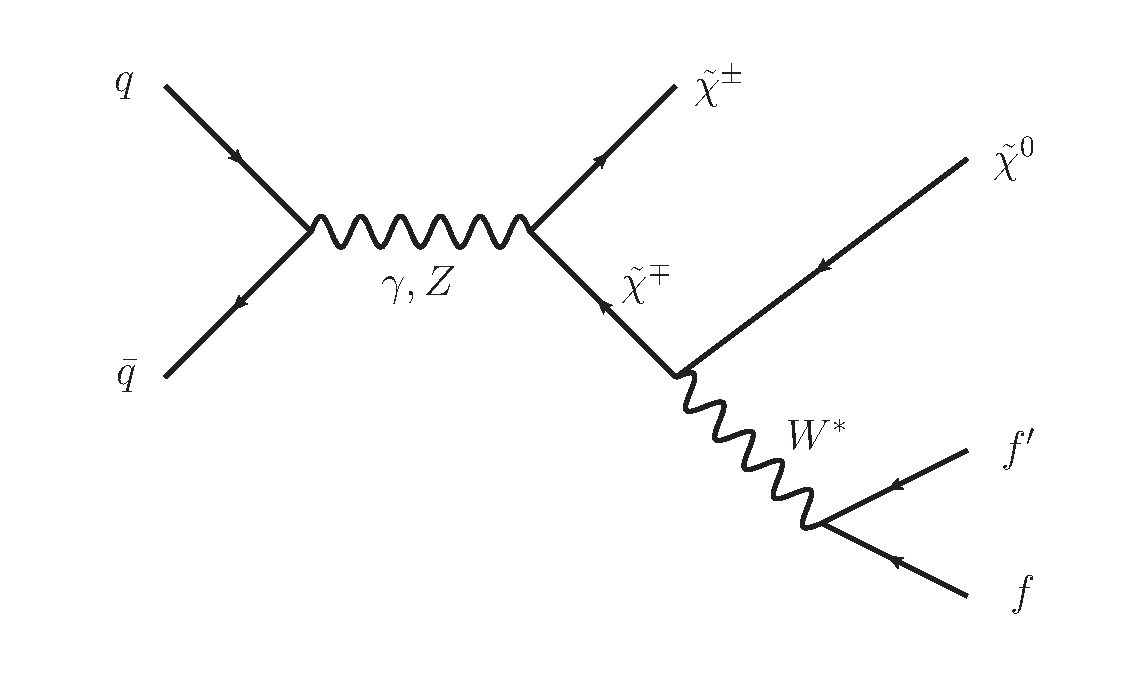
\includegraphics[width=0.75\textwidth]{figures/analysis/ChiChi_ProductionAndDecay.pdf}
  \end{tabular}
  \caption{Feynman diagram showing a possible production mechanism of a chargino pair and the decay channel of a chargino.}
  \label{fig:FeynmanDiagram}
\end{figure}

Other possible production channels are the exchange of a supersymmetric Higgs boson or via a t-channel squark exchange. 
The corresponding Feynman diagrams for the tree level production channels are shown in Fig.~\ref{fig:FeynmanDiagramProductionCharginoPair}.

\begin{figure}[!b]
  \centering 
  \begin{tabular}{c}
    \frame{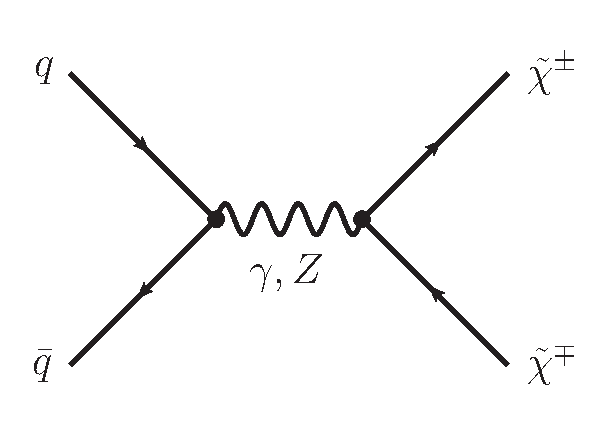
\includegraphics[width=0.33\textwidth]{figures/analysis/ChiChi_GammaZ.pdf}
    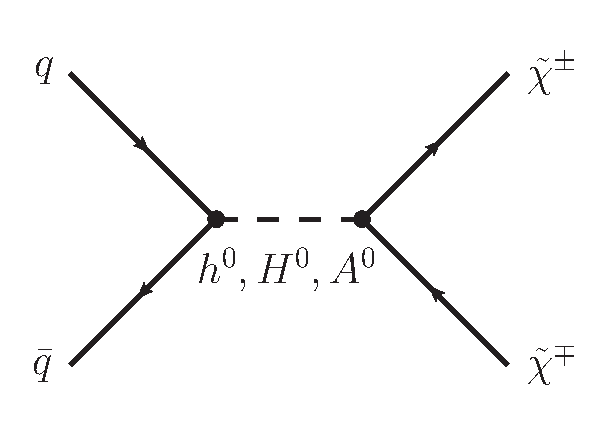
\includegraphics[width=0.33\textwidth]{figures/analysis/ChiChi_Scalar.pdf}
    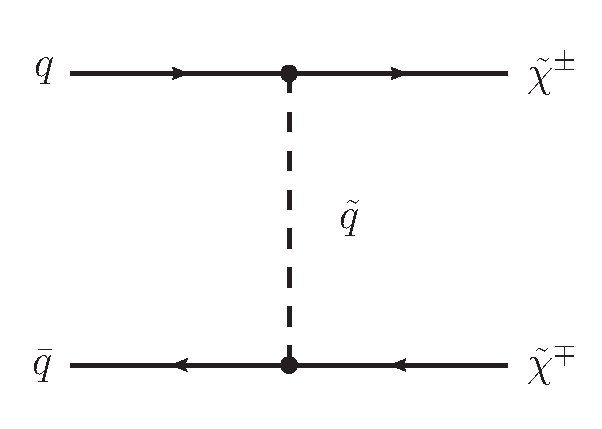
\includegraphics[width=0.33\textwidth]{figures/analysis/ChiChi_Squark.pdf}}
  \end{tabular}
  \caption{Main tree level diagrams for chargino pair production.}
  \label{fig:FeynmanDiagramProductionCharginoPair}
\begin{tabular}{c}
    \frame{    
    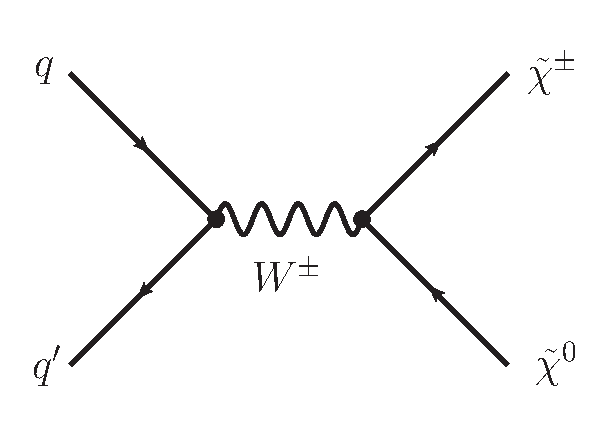
\includegraphics[width=0.33\textwidth]{figures/analysis/ChiChi0_WBoson.pdf}
    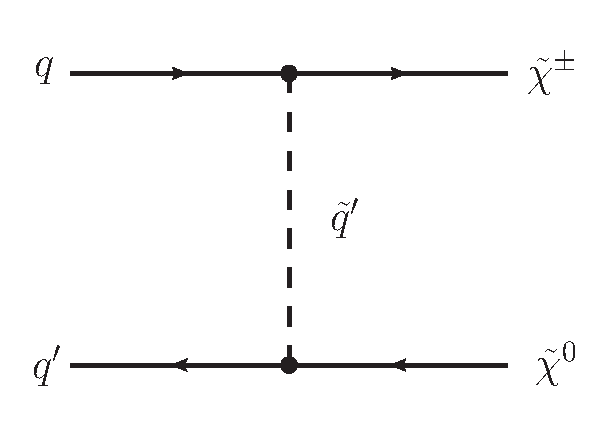
\includegraphics[width=0.33\textwidth]{figures/analysis/ChiChi0_Squark.pdf}
    }
  \end{tabular}
  \caption{Main tree level diagrams for chargino neutralino production.}
  \label{fig:FeynmanDiagramProductionCharginoNeutralino}
\end{figure}
Another possibility of chargino production is the chargino neutralino production channel. 
On tree level, there exist two production mechanism: the s-channel W boson exchange and the t-channel squark exchange, see Fig.~\ref{fig:FeynmanDiagramProductionCharginoNeutralino} for the Feynman diagrams.\\

Even if the presented supersymmetric model where $\chi^{\pm}_1$ and $\chi^{0}_1$ are nearly mass-degenerate leads to more exotic signatures at the CMS experiment, there have been already several analyses conducted in CMS which are in principle (even not all were designed to be) sensitive to these models.
Among those are a search for long-lived charged particles \cite{bib:CMS:HSCP_8TeV}, which was mainly designed for particles which have such a long lifetime that they travel through the full detector without decaying and a search for disappearing tracks \cite{bib:CMS:DT_8TeV} which looked for rather intermediate lifetimes, where the charginos decays already inside the tracker. 
Within \cite{bib:CMS:DT_8TeV}, a study was done, based on an interpretation exercise \cite{bib:CMS:HSCPReinterpreation_PAS} within the phenomenological MSSM (see Sec.~\ref{theorySUSY} for a detailed introduction to the pMSSM), which tests the exclusion power of various analyses done at CMS.

\begin{figure}[!b]
  \centering 
  \begin{tabular}{c}
    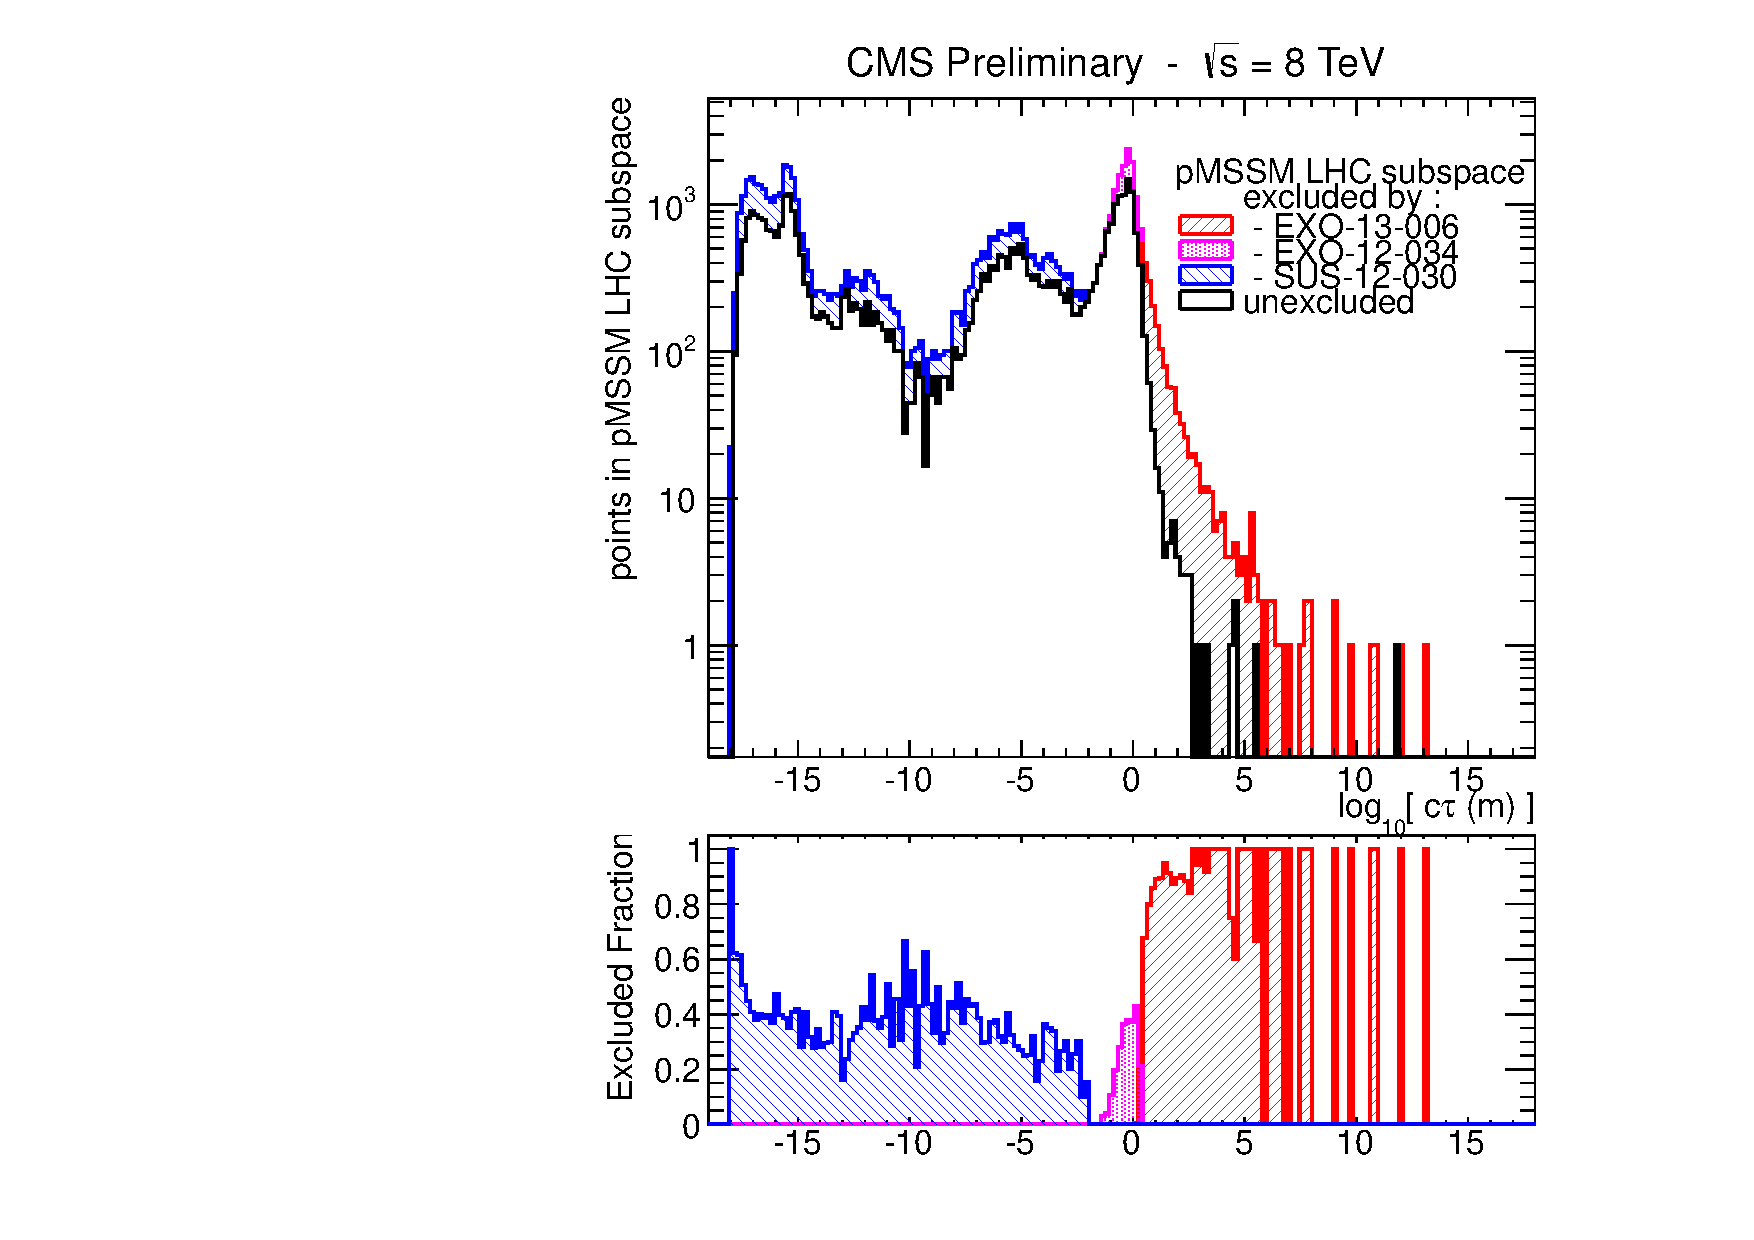
\includegraphics[width=0.75\textwidth]{figures/analysis/pMSSM_vs_ctau.pdf}
  \end{tabular}
  \caption{Exclusion power of various analyses dependent on chargino lifetime [c$\tau$]. Lower part of the plot shows the excluded fraction. Taken from: \href{https://twiki.cern.ch/twiki/bin/view/CMSPublic/PhysicsResultsEXO12034}{click here}.}
  \label{fig:pMSSMplot}
\end{figure}
In Fig.~\ref{fig:pMSSMplot}, the exclusion power of the search for long-live charged particles \cite{bib:CMS:HSCP_8TeV} in red, the search for diasappearing tracks \cite{bib:CMS:DT_8TeV} in purple and a collection of various SUSY analysis from \cite{bib:CMS:pMSSMinterpretation_7TeV_PAS} in blue over the chargino mass is shown. 
In black the distribution of the unexcluded pMSSM parameter points vs. the chargino mass can be seen.
The sampling of the parameter space points was done according to a pre-CMS likehood function, which takes into account electroweak precisicion measurements, etc.
In the lower part of Fig~\ref{fig:pMSSMplot}, the excluded fraction of pMSSM points is shown. 
It can be seen, that the more general SUSY searches are mostly sensitive to shorter chargino lifetimes ($c\tau \lesssim 10 \,\text{cm}$), whereas the search for long-lived particles shows very good sensitivity for lifetimes $>100\,$cm.
The search for disappearing tracks is sensitive on supersymmetric models with chargino lifetimes between $35\,\text{cm} \lesssim c\tau \lesssim 100\,\text{cm}$.

This analysis is targeting the gap between the disappearing track search (purple area) and the searches which are sensitive to instanteanously decaying charginos (blue area). The idea is to make use of the variable dE/dx which can be very discriminating for particles with high mass.
The challenges of such a search and the general strategy of this analysis will be presented int the next section.

%%%%%%%%%%%%%%%%%%%%%%%%%%%%%%%%%%%%%%%%%%%%%%%%%%%%%%%%%%%%%%%%%%%%%%%%%%%%%%%%%%%%%%%%%%%%%%%%%%%%%%%%%%%%%%%%%%%%%%%%%%%%%%%%%%%%%%%%%%%%%%%%%%%%%%%%%%%%%%%%%%%%%%%%%%%%%%%%%%%%
%%%%%%%%%%%%%%%%%%%%%%%%%%%%%%%%%%%%%%%%%%%%%%%%%%%%%%%%%%%%%%%%%%%%%%%%%%%%%%%%%%%%%%%%%%%%%%%%%%%%%%%%%%%%%%%%%%%%%%%%%%%%%%%%%%%%%%%%%%%%%%%%%%%%%%%%%%%%%%%%%%%%%%%%%%%%%%%%%%%%
\section{General search strategy}
\label{sec:GeneralSearchStrategy}

When searching for supersymmetric models with long-lived \chipm, the strategy is of course highly dependent on the actual lifetime of the chargino. 
For long lifetimes, the chargino can reach the muon chambers and can be reconstructed as a muon (even with a longer time-of-flight). 
For lower lifetimes, the chargino can already decay inside the detector (e.g. the tracker), thus not leading to a reconstructed muon in the event, but only to an isolated track in the tracker. 
The detector signatures of these two scenarios are visualised in Fig~\ref{fig:CharginoPaiEventDisplay}, where in a cross-sectional view of the CMS detector simulated chargino-chargino events are shown.
\begin{figure}[!b]
  \centering 
  \begin{tabular}{c}
    \frame{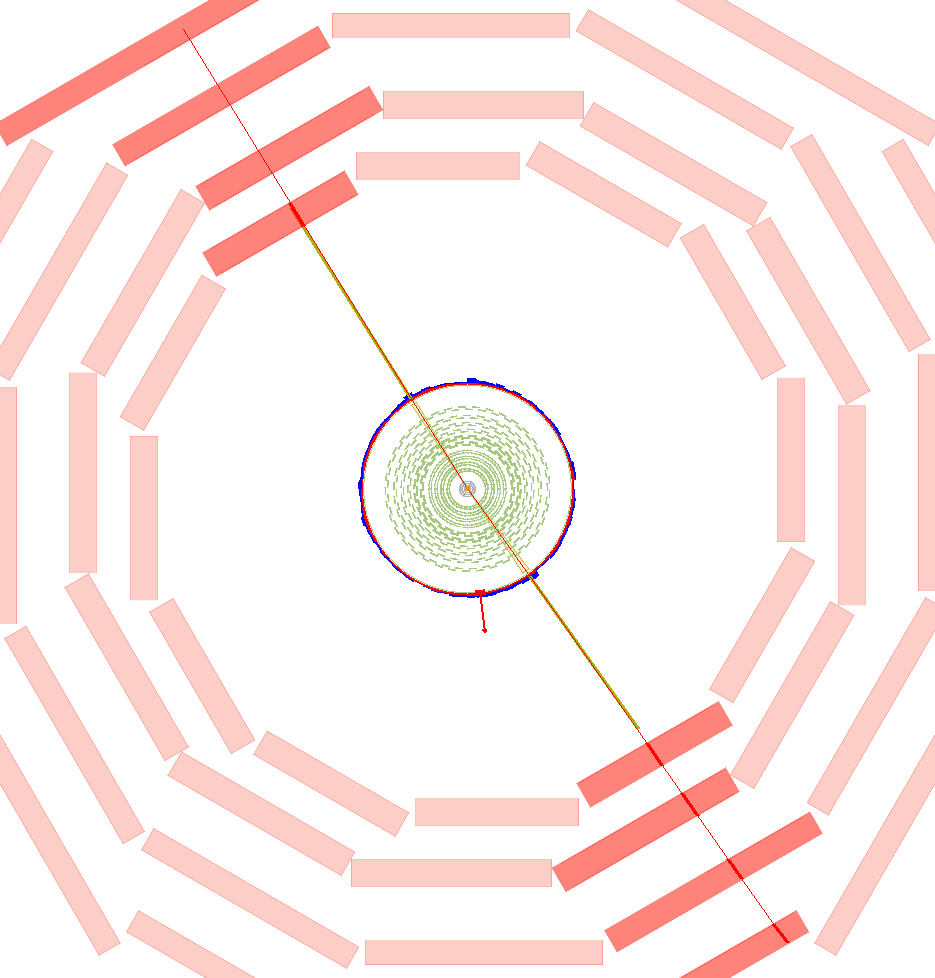
\includegraphics[width=0.31\textwidth]{figures/analysis/EventDisplay_scenario1.png}}
    \frame{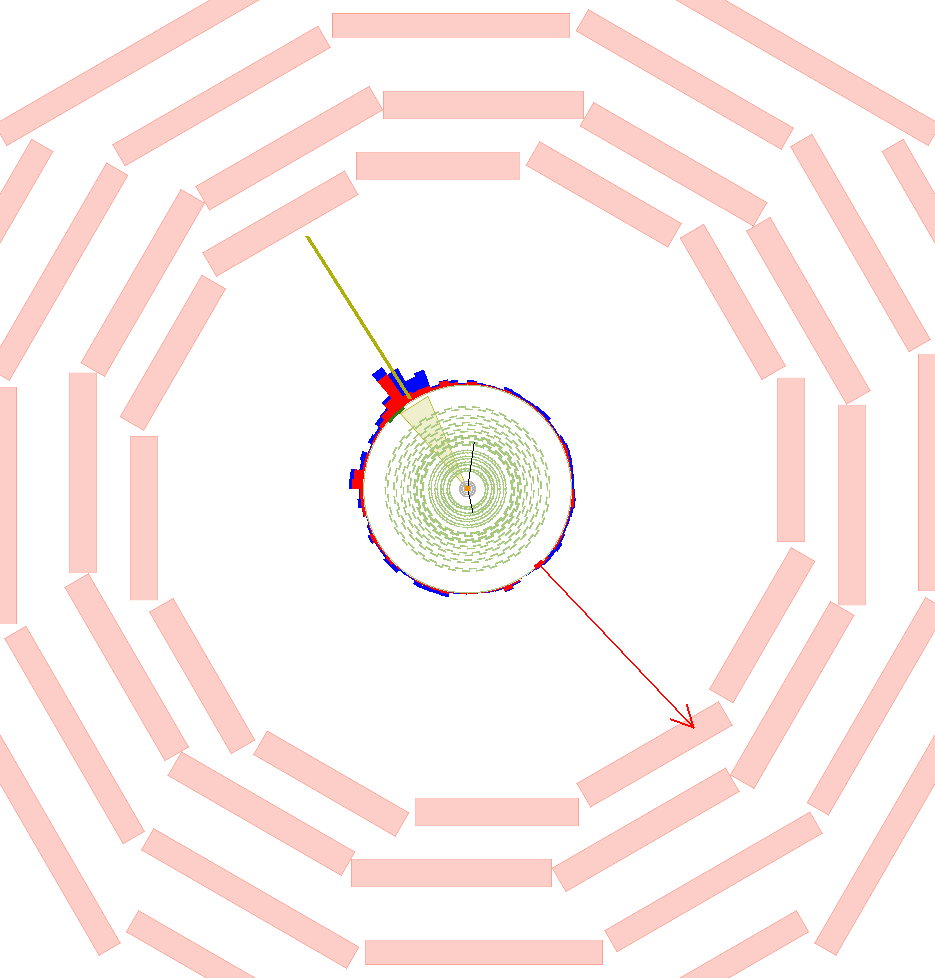
\includegraphics[width=0.31\textwidth]{figures/analysis/EventDisplay_scenario2.png}}
    \frame{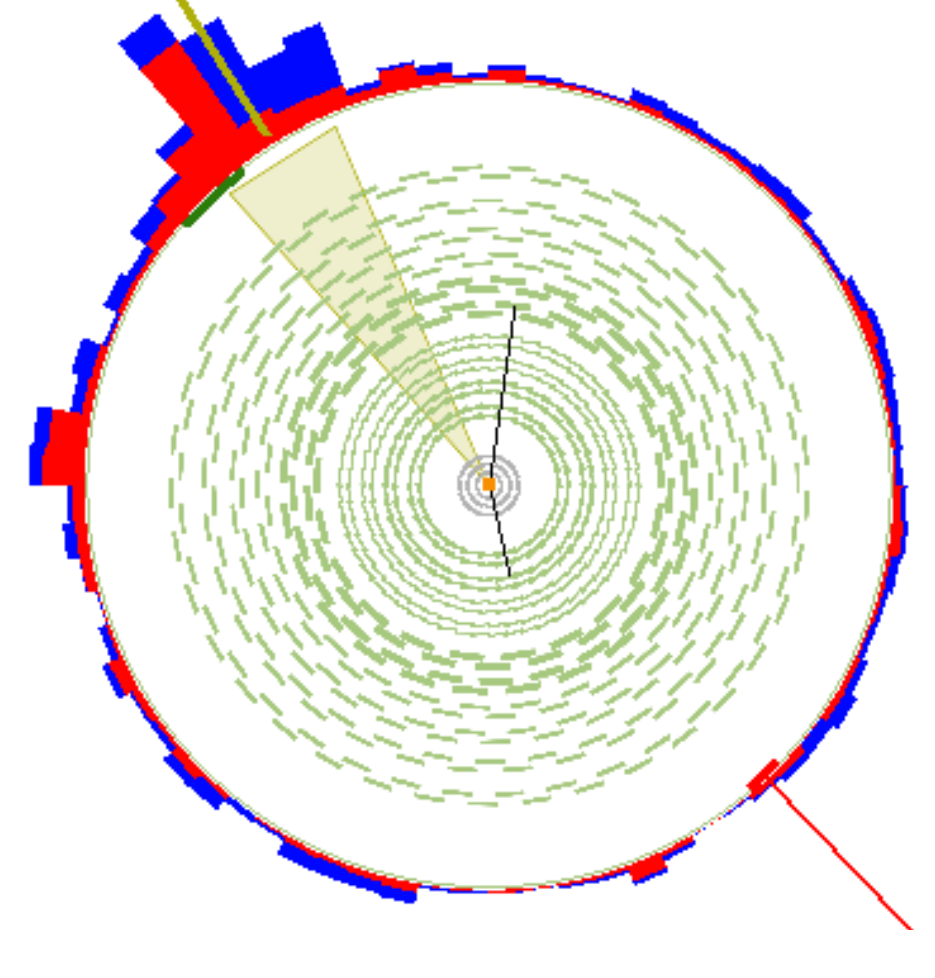
\includegraphics[width=0.31\textwidth]{figures/analysis/EventDisplay_scenario2_Zoomed.png}}
  \end{tabular}
  \caption{Visualisation of possible signatures of a chargino pair produced with a lifetime of $c\tau = 10\,\text{m}$ (left) and a lifetime of $c\tau = 0.5\,\text{m}$ (middle and right). 
           In the left picture, both charginos are reconstructed as muons, which can be seen in the energy deposition in the muon chambers (red boxes). 
           In the middle picture both charginos are only visible as tracks in the tracker (black lines), where both trajectories end inside the silicon tracker, showing the decay point point of the corresponding chargino. 
           The right picture is a zoom of the picture in the middle. Here only the cross-section of the tracker (green wavy lines) is displayed. The red arrow shows the missing transverse energy in the event.} 
  \label{fig:CharginoPaiEventDisplay}
\end{figure}
As mentioned before, this analysis targets a search for supersymmetry with charginos of lifetimes between $10\,\text{cm} \lesssim c\tau \lesssim  40\,\text{cm}$.
That means that the charginos decay rather early in the detector, even at the beginning of the tracker. 
The distinct challenges of such an analysis, shall be listed in the following passage.

First of all, in case R-parity (see Sec.~\ref{theorySUSY}) is conserved, one of the decay products of the chargino, which is the lightest neutralino \chiO is stable, thus travelling through the whole detector only weakly intereacting.
Therefore it is not detectable. 
The other chargino decay product, e.g. a pion, can be hardly reconstructed, mainly because it does not origin from the primary vertex (if the chargino reaches the detector before its decay), 
but secondarily because it is very low in momentum because of the mass-degeneracy between \chipm and \chiO.
The momentum of the decay product is of course highly dependent on the actual mass gap between the neutralino and the chargino.
A typical \pt distribution of a pion originating from a chargino decay can be found in Fig.~\ref{fig:KinkedTrack} for a mass gap between \chipm and \chiO of 150\,\mev.
\begin{figure}[!t]
  \centering 
  \begin{tabular}{c}
    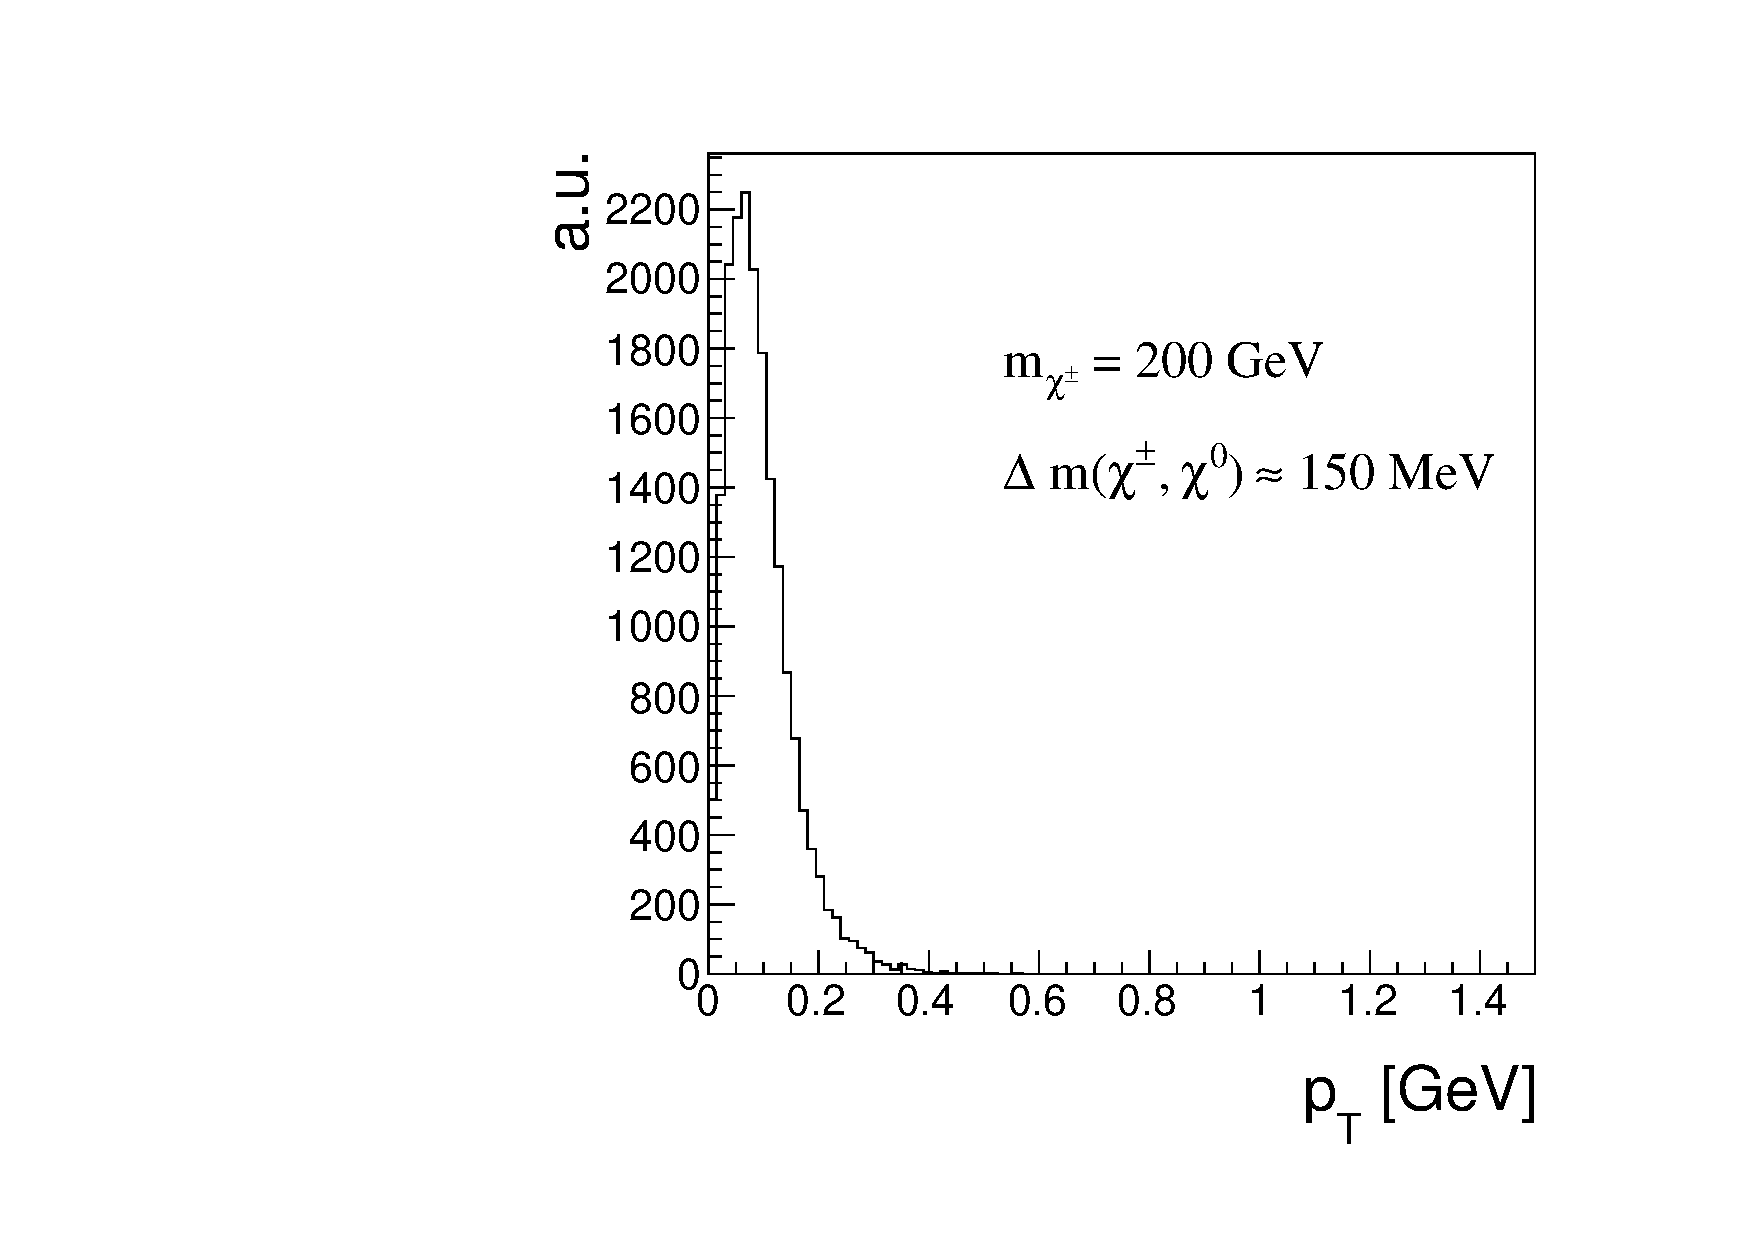
\includegraphics[width=0.6\textwidth]{figures/analysis/ptOfPions.pdf}
  \end{tabular}
  \caption{Transverse momentum distribution of pions coming from chargino decay into a neutralino with a mass gap of 150\mev.}
  \label{fig:ptOfPions}
\end{figure} 
The \pt distribution peaks at \mbox{$\sim$ 100\,\mev} and ends at \mbox{\pt $\sim 400\,$\mev}.
When the transverse momentum of a particle is very low, the particle trajectory is much more bended compared to a particle with higher \pt (see Fig.~\ref{fig:KinkedTrack} for illustration), 
thus making the detection of such a particle very challinging.
\begin{figure}[!bt]
  \centering 
  \begin{tabular}{c}
    \frame{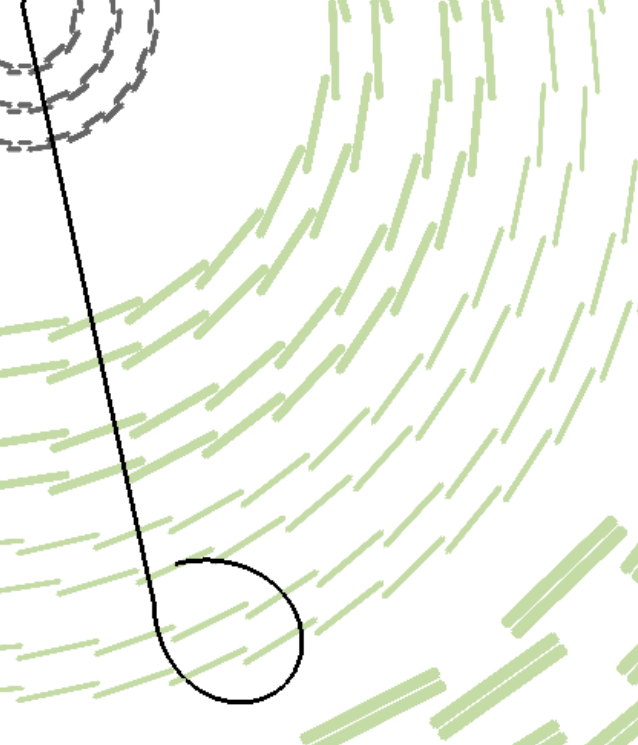
\includegraphics[width=0.3\textwidth]{figures/analysis/KinkedTrackZoom.png}}
  \end{tabular}
  \caption{Cross-sectional view of the tracker (different tracker layers are illustrated with wavy green lines) and a simulated chargino track (black line) decays to a pion (bended black line).}
  \label{fig:KinkedTrack}
\end{figure} 
Because of the stronger bending, the track reconstruction efficiency decreases for particles with a transverse momentum below 1\,\gev rapidely, ending at around 40\% for isolated pions with a \pt of 100\mev (see \cite{bib:CMS:tracking_8TeV}).

Taking the hard or even impossible detection of the decay products of the chargino, this lead to the fact, that besides the (short) track of the chargino, nothing can be seen in the detector.
Unfortunately, there is no dedicated track trigger at CMS, which makes a specific detection of those events with the help of the chargino track impossible.
To be able to search for these models, one therefore need to take advantage of higher order contributions to the feynman diagrams shown in the previous sections (Figs.~\ref{fig:FeynmanDiagramProductionCharginoPair},\ref{fig:FeynmanDiagramProductionCharginoNeutralino}), resulting in initial state radiation (ISR).
When the initial quarks radiate a high \pt gluon, the resulting jet can be detected and can offer a possibility to search for isolated tracks in the tracker.
The non-detection of the chargino's decay products plus a high \pt ISR jet lead additionally to missing transverse energy (MET) in the event. 
Exploiding these two circumstances, it is possible to detect chargino-pair or chargino-neutralino events with the help of Jet+MET triggers.\\

To select possible charginos in an event, additional requirements for isolated, high \pt tracks are needed.
Those tracks can be eventually disappearing, which means that the track does not cross the full pixel and strip detector.
This can happen, when the chargino decays inside the tracker.
For very low lifetimes, the tracks can be very short and can have only a few hits in the detector. 
To define a helical path five parameters are needed, therefore a minimum of three hits are required to be able to reconstruct a particle's trajetcory (see \cite{bib:CMS:tracking_8TeV}).
In this analysis, the massiveness of the charginos shall be exploited, on the one hand by selecting only high \pt tracks, but on the other hand by requiering a high energy deposition per path length (\dedx).
The energy deposition depends quadratically on the particle's mass for low velocities ($0.2<\beta\gamma<0.9$).
\begin{equation}
\langle\frac{dE}{dx}\rangle = K \frac{m^2}{p^2} +C
\end{equation}

thus constitute a very nice discriminating variable for massive particles. 
A specific challenge for this analysis is the combinitation of searching for short tracks and utilising the energy deposition of the chargino.
Unfortunately, the pixel tracker during Run I underwent only a calibration procedure at the very beginning of the start of data taking in 2011.
Because of various readjustments during the year 2012, this introduced a huge non-calibration over time. 
In case we want to look at the \dedx of the tracks, there is therefore the need to recalibrate the pixel detector in order to be able to use its energy information in this analysis.

%\begin{itemize}
%\item No detection of low momentum fermions possible (fermion pt plot?), no detection of the decay products
%\item Concentration on intermediate lifetime $\rightarrow$ only a (short) chargino track can be seen.
%\item Show event displays and sketch for pion decyay!
%\item Detection via ISR 
%\item Event selection by ISR jet and MET
%\item Detection of track (possibly short and disappearing and highly ionizing, not reconstructed as muon)
%\item Short and highly ionizing track $\rightarrow$ inclusion of pixel tracker information 
%\end{itemize}

\subsection{Comparison to existing searches}
As already mentioned before, there were several analyses at CMS, which are sensitive to intermediate lifetime charginos. 
Most notably, the search for long lived-charged particles \cite{bib:CMS:HSCP_8TeV} and the search for disappering tracks \cite{bib:CMS:DT_8TeV}.
An improvement in sensitivity to shorter lifetimes compared to these analysis shall be achieved by including also very short tracks in this analysis.
In \cite{bib:CMS:HSCP_8TeV}, a minimum number of eight hits, whereas in \cite{bib:CMS:DT_8TeV} a minimum of seven hits are required. 
This can be very unefficient for shorter lifetimes, where most of the charginos decay already after the pixel tracker ($\sim 10\,\text{cm}$).
Additionally, the search for disappearing tracks does not make use of the high energy deposition of heavy particles. 
On the other hand is this variable used in the search for long-lived particles, where the sensitiviy decreases much quicker for shorter lifetimes (see Fig~\ref{fig:pMSSMplot}).
In \cite{bib:CMS:DT_8TeV}, there is a muon-veto exploited to supress SM background coming from processes resulting in one or two muons. 
Additionnally, it requires missing outer hits in the tracker (disappearing track), which makes this analysis especially sensitive to a shorter tracks.
In the preseneted analaysis, the stron selection on the number of hits in the tracker shall be lowered and the variable \dedx shall be included to increase sensitiviy.
Also, a muon-veto is applied to make the selection expecially sensitive to very short lifetimes.
\textcolor{red}{MAYBE} show here already a plot with the number of valid hits distribution to emphasize the importance of lossening the number of hits cut!
%%%%%%%%%%%%%%%%%%%%%%%%%%%%%%%%%%%%%%%%%%%%%%%%%%%%%%%%%%%%%%%%%%%%%%%%%%%%%%%%%%%%%%%%%%%%%%%%%%%%%%%%%%%%%%%%%%%%%%%%%%%%%%%%%%%%%%%%%%%%%%%%%%%%%%%%%%%%%%%%%%%%%%%%%%%%%%%%%%%%
%%%%%%%%%%%%%%%%%%%%%%%%%%%%%%%%%%%%%%%%%%%%%%%%%%%%%%%%%%%%%%%%%%%%%%%%%%%%%%%%%%%%%%%%%%%%%%%%%%%%%%%%%%%%%%%%%%%%%%%%%%%%%%%%%%%%%%%%%%%%%%%%%%%%%%%%%%%%%%%%%%%%%%%%%%%%%%%%%%%%
\section{Improved dE/dx measurement of short tracks}
\label{sec:DeDxMeasurement}
It was already pointed out, that the inclusion of the pixel energy measurements can increase the sensitivity when searching especially for short tracks.
While the silicon strip detetcor has already been calibrated as part of the search for long-lived charged particles \cite{bib:CMS:HSCP_8TeV}, there was never an offline calibration done for the pixel silicon tracker.
To increase the discrimination power of \dedx, such an calibration procedure was therefore conducted within this PHD thesis.
 
\subsection{Measuring dE/dx}
The mean energy loss per path length of particles travelling through a layer of material can be described with the Bethe-Bloch formula \cite{bib:Bethe_1930,bib:Bloch_1933}:
\begin{equation}
\langle \frac{dE}{dx} \rangle = kz^2\frac{Z}{A}\frac{1}{\beta^2} [ \frac{1}{2} \ln{\frac{2m_e c^2 \beta^2 \gamma^2 T_{\text{max}}}{I^2}} - \beta^2 - \frac{\delta( \beta \gamma )}{2} ].
\end{equation}
It is valid, where the main energy loss originates from ionization effects which is in a region between $0.1\lesssim\beta\gamma\lesssim 1000$.
It is a function of the atomic number ($Z$) and the atomic mass of the absorber ($A$). 
The mean excitation energy ($I$) for silicon is 173$\pm$3\,eV \cite{?}. 
$T_{\text{max}}$ stands for the maximum energy transfer in a single collision.
The relevant particle's properties are the velocity ($\beta$), the lorentz factor ($\gamma$) and the charge (z) of the incident particle.
The density correction $\delta( \beta \gamma )$ reduces the mean energy loss at high energies because of polarization effects of the material.

Even if widely used, the Bethe-Bloch formula is ill-defined because of the use of the mean energy loss per path length.
The problem arises when looking at the fluctuations of a particle's energy deposition.
In case particles cross material layers of moderate sickness, the probability density function of the deposited energy can be described by a Landau function \cite{bib:Landau_1944}. 
The Landau distribution is a highly asymmetric distribution with a long tail torwards the right end (see Fig.~\ref{fig:landau}).
Theoretically it extends to infinite energies, however in nature the maximal deposited energy is of course limited by the particle's full energy.
\begin{figure}[!t]
  \centering 
  \begin{tabular}{c}
  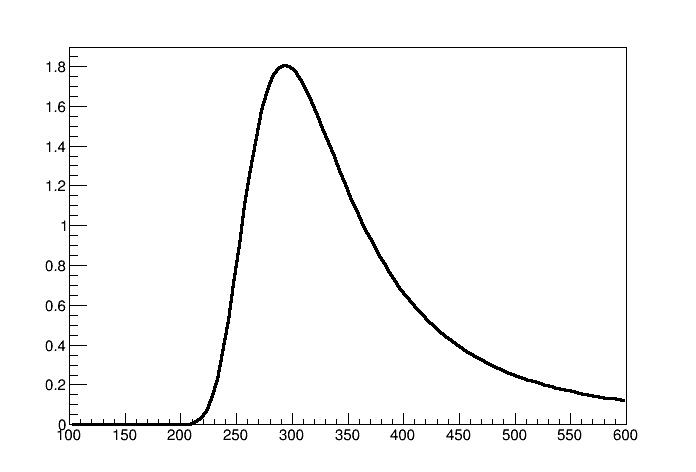
\includegraphics[width=0.5\textwidth]{figures/analysis/landau.png}
  \end{tabular}
  \caption{Illustration of a Landau function. Parameters were arbitrarily chosen for this figure.} 
  \label{fig:landau}
\end{figure}
The mean and the variance of a landau distribution are not defined. 
This is again different for a (limited) measurment, as there it is always possible to calucalute a mean.
Still, this leads to the fact that the definition of the mean energy loss per path length is a problematic and unstable concept.
A much better observable is the most probably value (MPV) being the maximum of the landau function, which is much more stable compared to the mean. 
The most probable energy loss of a charged particle is defined by the Landau-Vavilov-Bichsel equation:
\begin{equation}
\Delta_p = \xi \left[ \ln \frac{2mc^2\beta^2\gamma^2}{I}  + \ln\frac{\xi}{I} + j - \beta^2 - \delta(\beta\gamma)  \right],
\end{equation}
where $\xi=(K/Z)\langle Z/A \rangle (x/\beta^2)$. 
The thickness of the absorber $x$ appears explicitly in the Landau-Vavilov-Bichsel equation making the most probable energy loss per path \mbox{length $\frac{\Delta_p}{dx}$} logarithmically dependent on $x$.
A comparison between the Bethe mean energy loss $\langle \frac{dE}{dx} \rangle$ and the most probable energy loss $\frac{\Delta_p}{dx}$ are shown in Fig.~\ref{fig:dEdx_Bethe_Landau}.
\begin{figure}[!bt]
  \centering 
  \begin{tabular}{c}
  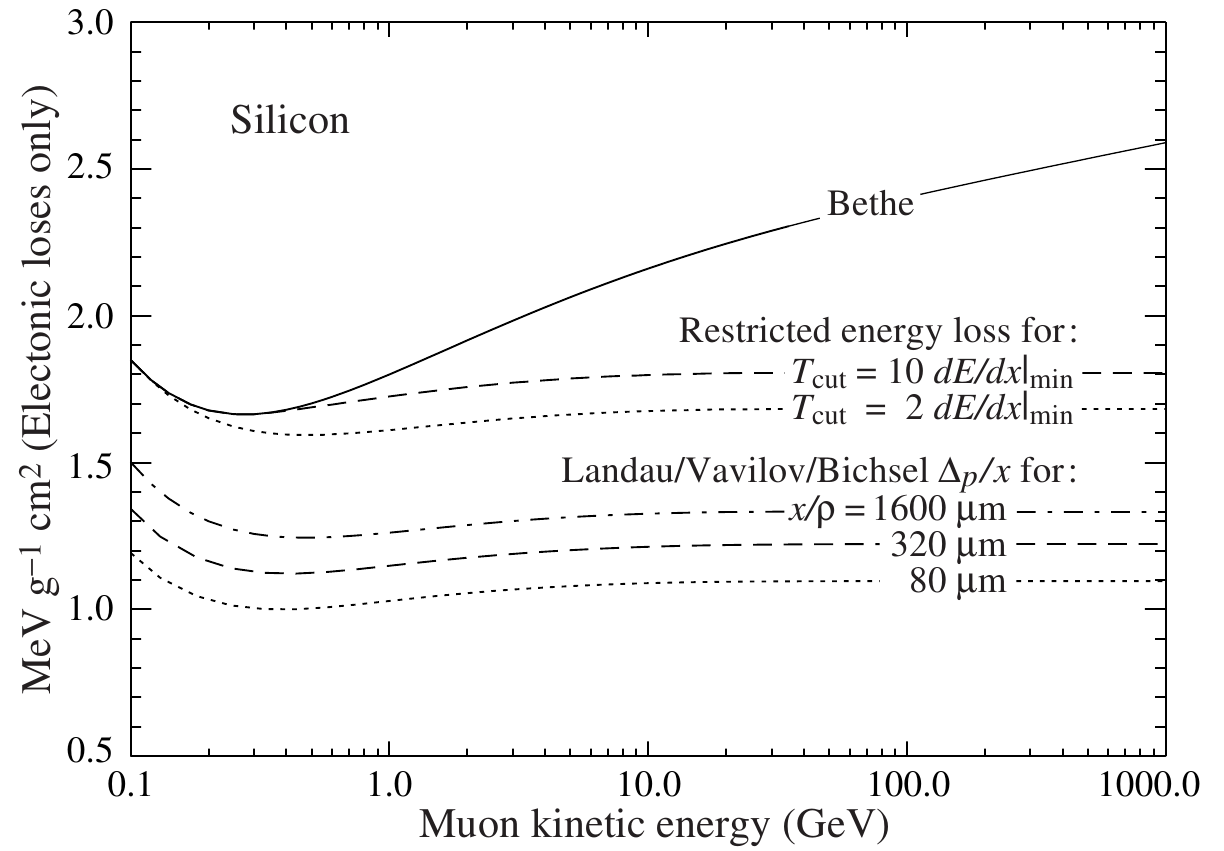
\includegraphics[width=0.5\textwidth]{figures/analysis/dEdx_Bethe_Landau.png}
  \end{tabular}
  \caption{Comparison between the Bethe mean energy loss with and without restricted energy loss and the most probable energy loss described by the Landau-Vavilov-Bichsel function for different sizes of thickness. 
           Taken from \cite{bib:PDG_2014}.} 
  \label{fig:dEdx_Bethe_Landau}
\end{figure}
\\

SM particles as pions and muons are minimal ionising in silicon for $\beta\gamma \sim 4$, dependent on the thickness of the material (see Fig.~\ref{fig:dEdx_Landau_Silicon} ). 
For higher momenta the deposited energies increase again reaching a plateau at around $\beta\gamma\sim100$. 
However, new heavy charged particles would mainly be unrelativistic because of their high mass and would therefore deposit much higher energies in the detector.
This makes the energy deposition per path length to a very well discriminating variable.
\begin{figure}[!bt]
  \centering 
  \begin{tabular}{c}
  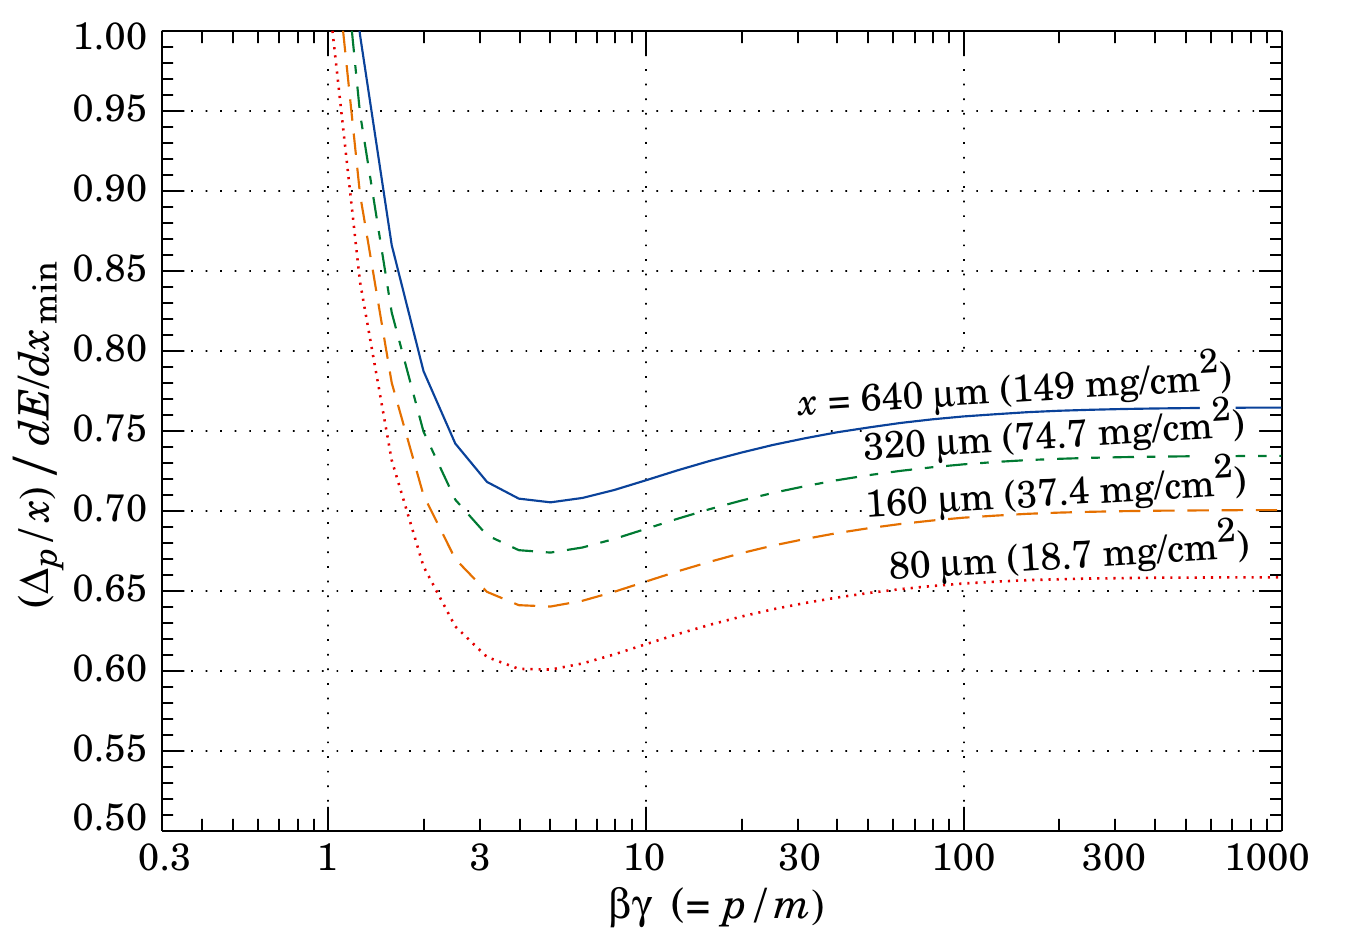
\includegraphics[width=0.5\textwidth]{figures/analysis/dEdx_Landau_Silicon.png}
  \end{tabular}
  \caption{Most probable energy loss in silicon, scaled to the mean loss of a minimal ionizing particle (388 eV/$\mu$m). Taken from \cite{bib:PDG_2014}.} 
  \label{fig:dEdx_Landau_Silicon}
\end{figure}
Thus, the energy loss per path length can be used to discriminate between SM particles and new heavy charged particles, which are usually unrelativistic because of their high mass.

%\begin{itemize}
%\item The variable dE/dx: General introdution
%\item Bethe-Bloch (difficult concept because of undefined mean of the Landau function)
%\item Landau distribution (no mean)
%\item Most probable energy loss landau vavilov function (show comparison plot Landau, Bethe)
%\item Minimal ionising particles (pt cut) (how dedx for pions CMS 2008)
%\end{itemize}

\subsection{Gain calibration of the silicon pixel tracker}

During Run I in 2012, the pixel silicon detector was continously subjected to an energy calibration, which is called gain calibration.
Every pixel was calibrated to the same response, such that the whole pixel tracker should be well inter-calibrated.
Unfortunately, due to imperfect constancy of the reference signal, the approximation of the atan() response with a linear function, and radiation and temperature induces changes, the energy calibration is not adequate to use the emasured energy deposition without further calibration.
This imperfection of the gain calibration can be seen in Fig.~\ref{fig:dEdx_beforeCalibration}, where the harmonic-2 estimator summed over all tracks  (see \cite{} for a detailed explanation) over time is shown.
Four different steps can be spotted. The first and the third correspond to a change  in the settings of the tracker, the second and fourth is, where a gain calibration was applied.
Unfortunately, although a gain calibration was applied (even with delay), it could not bring the average dE/dx to the same level before the change in the setting occured.
The size of the difference in the dE/dx measurement over time being around 10\% is too large to use the dE/dx out of the box.

\begin{figure}[!bt]
  \centering 
  \begin{tabular}{c}
  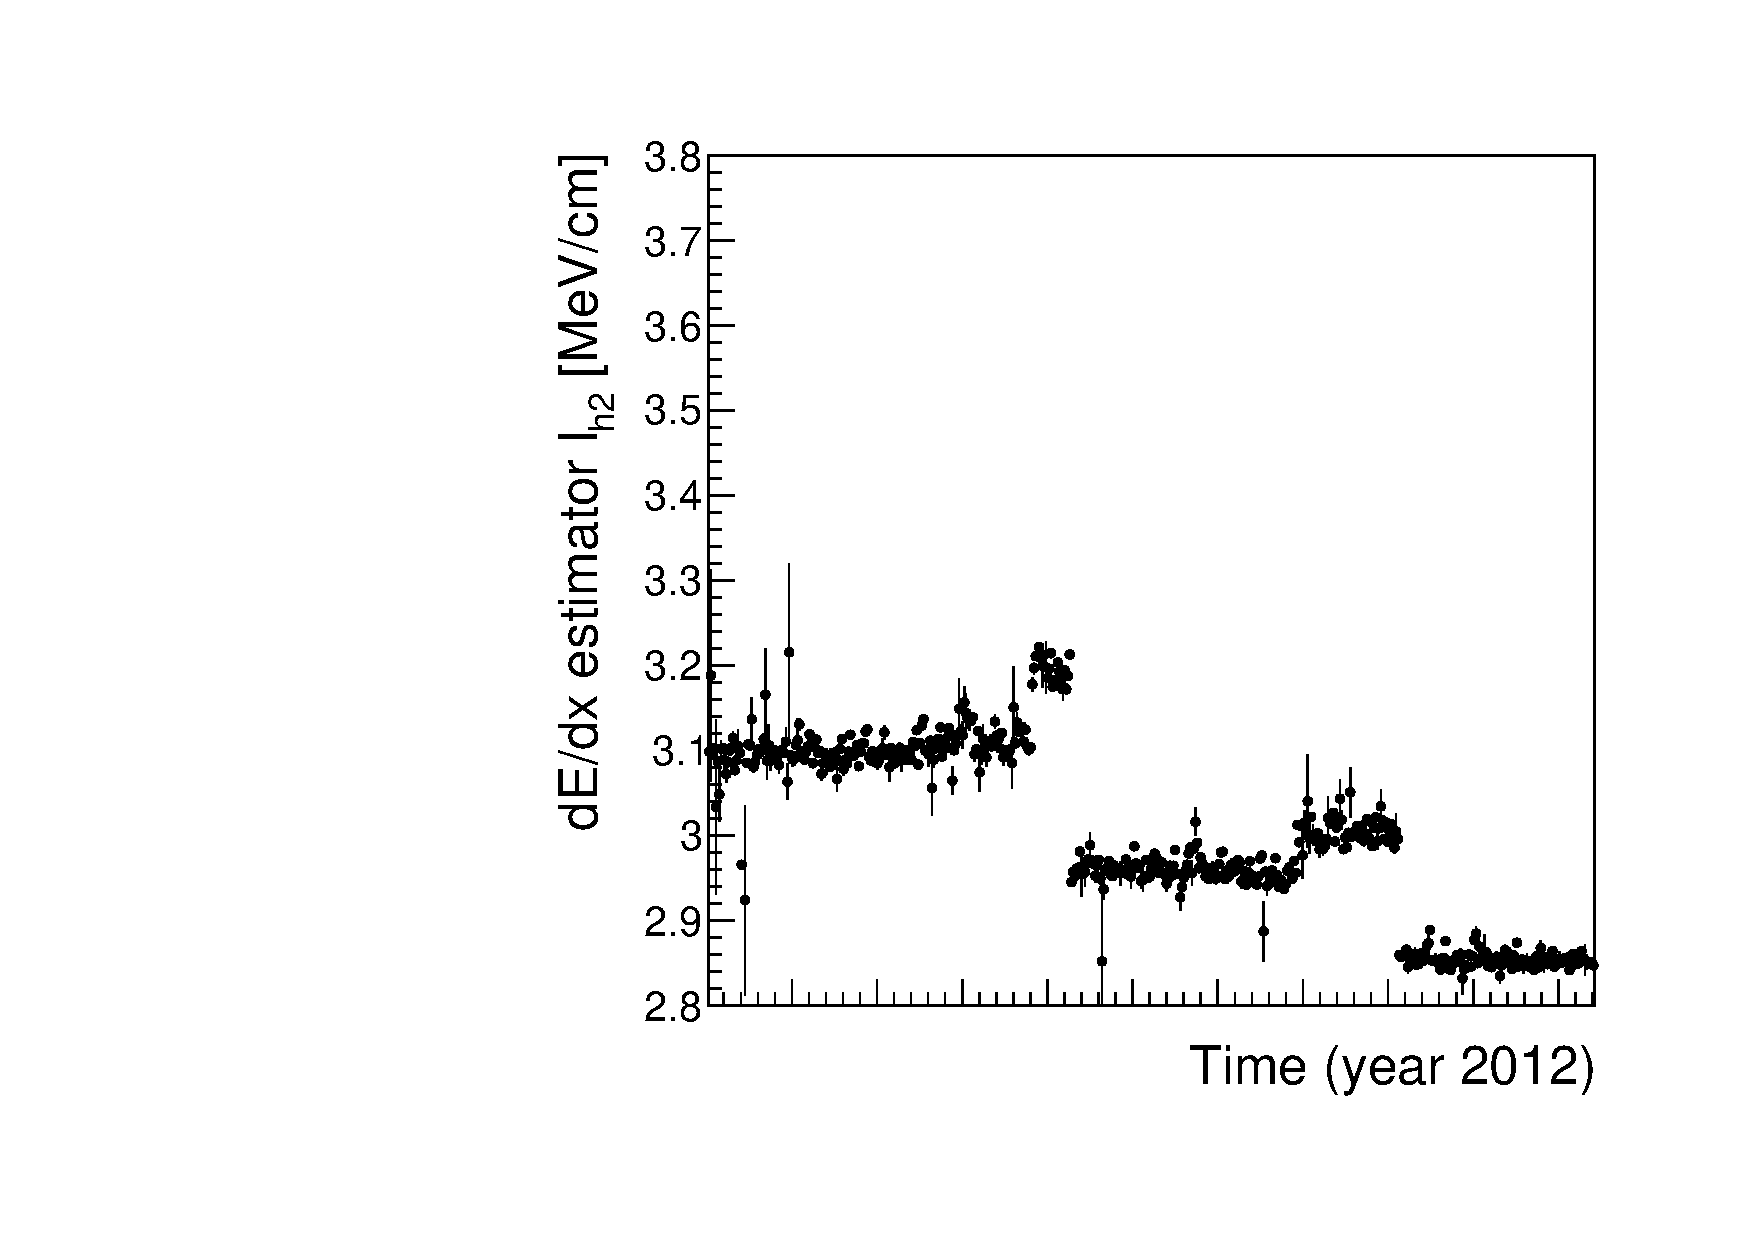
\includegraphics[width=0.5\textwidth]{figures/analysis/StabilityPlot_Pixel_beforeCalibration_withoutStepFits_NEW.pdf}
  \end{tabular}
  \caption{Sum of all track's dE/dx (harmonic-2 estimator) over the full year 2012. Every data point correspond to one run.} 
  \label{fig:dEdx_beforeCalibration}
\end{figure}

\begin{itemize}
\item What kind of calibrations are done with the silicon pixel and strip detectors?
\item Pixel detector has been calibrated once before ijecting it to CMS
\item dEdx not stable over time (show plot)
\item Describe the different levels of calibration (what is calibrated, pixels, what is not calibrated, ROC) (intercalibration of ROCs and a clibration vs. time)
\item How can the calibration been done (using MIPs, \pt cut, which samples are used - Min Bias samples)
\item Which validation procedure were conducted?
\item What are the results of the calibration
\end{itemize}

\subsection{Asymmetric Smirnov discriminator}

\subsection{Efficiency improvements}
%%%%%%%%%%%%%%%%%%%%%%%%%%%%%%%%%%%%%%%%%%%%%%%%%%%%%%%%%%%%%%%%%%%%%%%%%%%%%%%%%%%%%%%%%%%%%%%%%%%%%%%%%%%%%%%%%%%%%%%%%%%%%%%%%%%%%%%%%%%%%%%%%%%%%%%%%%%%%%%%%%%%%%%%%%%%%%%%%%%%
%%%%%%%%%%%%%%%%%%%%%%%%%%%%%%%%%%%%%%%%%%%%%%%%%%%%%%%%%%%%%%%%%%%%%%%%%%%%%%%%%%%%%%%%%%%%%%%%%%%%%%%%%%%%%%%%%%%%%%%%%%%%%%%%%%%%%%%%%%%%%%%%%%%%%%%%%%%%%%%%%%%%%%%%%%%%%%%%%%%%
\section{Simulated samples}
\label{sec:SimulatedSamples}
\subsection{SM samples}
\subsection{Signal samples}
%%%%%%%%%%%%%%%%%%%%%%%%%%%%%%%%%%%%%%%%%%%%%%%%%%%%%%%%%%%%%%%%%%%%%%%%%%%%%%%%%%%%%%%%%%%%%%%%%%%%%%%%%%%%%%%%%%%%%%%%%%%%%%%%%%%%%%%%%%%%%%%%%%%%%%%%%%%%%%%%%%%%%%%%%%%%%%%%%%%%
%%%%%%%%%%%%%%%%%%%%%%%%%%%%%%%%%%%%%%%%%%%%%%%%%%%%%%%%%%%%%%%%%%%%%%%%%%%%%%%%%%%%%%%%%%%%%%%%%%%%%%%%%%%%%%%%%%%%%%%%%%%%%%%%%%%%%%%%%%%%%%%%%%%%%%%%%%%%%%%%%%%%%%%%%%%%%%%%%%%%
\section{Event selection}
\label{sec:EventSelection}
\subsection{Datasets and triggers}
\begin{itemize}
\item Datasets and triggers used in the analysis
\item signal samples generated with Madgraph and pythia
\item They are decayed in Geant to only pions. Around ten different lifetimes were simulated
\item For other lifetimes: lifetime reweighting is done PLOT
\item For five diffenrent masses (100-500 GeV) 
\end{itemize}
\subsection{Preselection}
\begin{itemize}
\item Motivate different selection cuts
\item Reference DT search for most of them
\end{itemize}
\subsection{Main discriminating variables}
\begin{itemize}
\item dE/dx
\item pt
\item Show some MC signal bkg comparioson plots (only Wjets?)
\end{itemize}

%%%%%%%%%%%%%%%%%%%%%%%%%%%%%%%%%%%%%%%%%%%%%%%%%%%%%%%%%%%%%%%%%%%%%%%%%%%%%%%%%%%%%%%%%%%%%%%%%%%%%%%%%%%%%%%%%%%%%%%%%%%%%%%%%%%%%%%%%%%%%%%%%%%%%%%%%%%%%%%%%%%%%%%%%%%%%%%%%%%%
\section{Sources of backgrounds}
\label{sec:SourcesOfBackgrounds}
\begin{itemize}
\item Background consist of particles which make high energy deposits and are high pt
\item In general: Low background search
\end{itemize}
\subsection{Fake tracks}
\begin{itemize}
\item Definition of fake tracks
\item How can they fake the signal
\end{itemize}
\subsection{Muons}
\begin{itemize}
\item How can muons fake the signal
\end{itemize}
\subsection{Pions}
\begin{itemize}
\item How can pions fake the signal
\end{itemize}
\subsection{Electrons}
\begin{itemize}
\item How can electrons fake the signal
\end{itemize}
%%%%%%%%%%%%%%%%%%%%%%%%%%%%%%%%%%%%%%%%%%%%%%%%%%%%%%%%%%%%%%%%%%%%%%%%%%%%%%%%%%%%%%%%%%%%%%%%%%%%%%%%%%%%%%%%%%%%%%%%%%%%%%%%%%%%%%%%%%%%%%%%%%%%%%%%%%%%%%%%%%%%%%%%%%%%%%%%%%%%
%%%%%%%%%%%%%%%%%%%%%%%%%%%%%%%%%%%%%%%%%%%%%%%%%%%%%%%%%%%%%%%%%%%%%%%%%%%%%%%%%%%%%%%%%%%%%%%%%%%%%%%%%%%%%%%%%%%%%%%%%%%%%%%%%%%%%%%%%%%%%%%%%%%%%%%%%%%%%%%%%%%%%%%%%%%%%%%%%%%%
\section{Background estimation methods}
\label{sec:BackgroundEstimation}
\subsection{Fake background}
\subsection{Leptonic background}
\subsection{Systematic uncertainties}

%%%%%%%%%%%%%%%%%%%%%%%%%%%%%%%%%%%%%%%%%%%%%%%%%%%%%%%%%%%%%%%%%%%%%%%%%%%%%%%%%%%%%%%%%%%%%%%%%%%%%%%%%%%%%%%%%%%%%%%%%%%%%%%%%%%%%%%%%%%%%%%%%%%%%%%%%%%%%%%%%%%%%%%%%%%%%%%%%%%%
\section{Optimization of search sensitivity}
\label{sec:Optimization}
\begin{itemize}
\item Show plots
\item show table
\item Include NlostOuter here, too
\end{itemize}

%%%%%%%%%%%%%%%%%%%%%%%%%%%%%%%%%%%%%%%%%%%%%%%%%%%%%%%%%%%%%%%%%%%%%%%%%%%%%%%%%%%%%%%%%%%%%%%%%%%%%%%%%%%%%%%%%%%%%%%%%%%%%%%%%%%%%%%%%%%%%%%%%%%%%%%%%%%%%%%%%%%%%%%%%%%%%%%%%%%%
\section{Statistical Methods/ Limit setting}
\label{sec:LimitSetting}

%%%%%%%%%%%%%%%%%%%%%%%%%%%%%%%%%%%%%%%%%%%%%%%%%%%%%%%%%%%%%%%%%%%%%%%%%%%%%%%%%%%%%%%%%%%%%%%%%%%%%%%%%%%%%%%%%%%%%%%%%%%%%%%%%%%%%%%%%%%%%%%%%%%%%%%%%%%%%%%%%%%%%%%%%%%%%%%%%%%%
\section{Results}
\label{sec:Results}
\begin{itemize}
\item Data cutflowtable
\item Tables with results
\item One plot (4 bins: Prediction and data)
\end{itemize}

%%%%%%%%%%%%%%%%%%%%%%%%%%%%%%%%%%%%%%%%%%%%%%%%%%%%%%%%%%%%%%%%%%%%%%%%%%%%%%%%%%%%%%%%%%%%%%%%%%%%%%%%%%%%%%%%%%%%%%%%%%%%%%%%%%%%%%%%%%%%%%%%%%%%%%%%%%%%%%%%%%%%%%%%%%%%%%%%%%%%
\section{Interpretation}
\label{sec:Interpretation}
\subsection{Systematic uncertainties of simulated signal samples}
\subsection{Exclusion limits}
\begin{itemize}
\item 1-d limits
\item 2-d limits
\end{itemize}

